\section{Experiments}
\subsection{Sea surface height and velocities}

\textbf{(i, ii)} Steady state for a numerical solution means that the solution does not change with time, i.e. $\partial/\partial t = 0$ or $h^{n+1}\approx h^n$. Thus a steady state solution means that the free surface height ($\eta$) velocities ($u,v$) and the energies ($EK, EP, E_\text{tot}$) do not change with time. In the geostrophic adjustment problem, the steady state solution is given by \autoref{eq:solh} and \autoref{eq:solv}, where one can see tha there is no time dependence. Thus, the solution is a steady state solution. In the experiment this is however measured when the next time step does not change the solutions, i.e 
\[
\begin{pmatrix}
\eta^{n+1} \\
u^{n+1} \\
v^{n+1} \\
E^{n+1}
\end{pmatrix}
\approx
\begin{pmatrix}
\eta^{n} \\
u^{n} \\
v^{n} \\
E^{n}
\end{pmatrix}
\]

Thus one can identify if steady state is not yet reached by observing the time evolution of the free surface height, velocities and energies. If these quantities are still changing with time, by oscillations or by a trend, then the solution has not yet reached steady state. One can also compare the numerical solution to the analytical solution at different time steps, and if they are not close to each other, then the solution has not yet reached steady state or the numerical solution is not accurate.

\textbf{(iii)} The initial state of the model, the first few hours and the final state can be seen in \autoref{fig:graph}. One can see that during the first hours the model is adjusting from the initial condition, and the free surface height and velocities are changing with time. One can see fast moving waves moving away from the center out towards the edge. One can also see how the sponge 'eats' some of the waves. However all fast waves are not eaten by the sponge, as seen between hour 4 and 4.5 where a reflection can be seen. This is thus a source of error in the model, which prevents the model from reaching a steady state quickly. Better solutions could be observed with a thicker sponge, however, this would just give a thinner area to plot. Thus one can observe how the model is adjusting to geostrophy. This can also be seen in \autoref{fig:im}--\ref{fig:gaussian}.

\begin{figure}[H]
    \centering    
    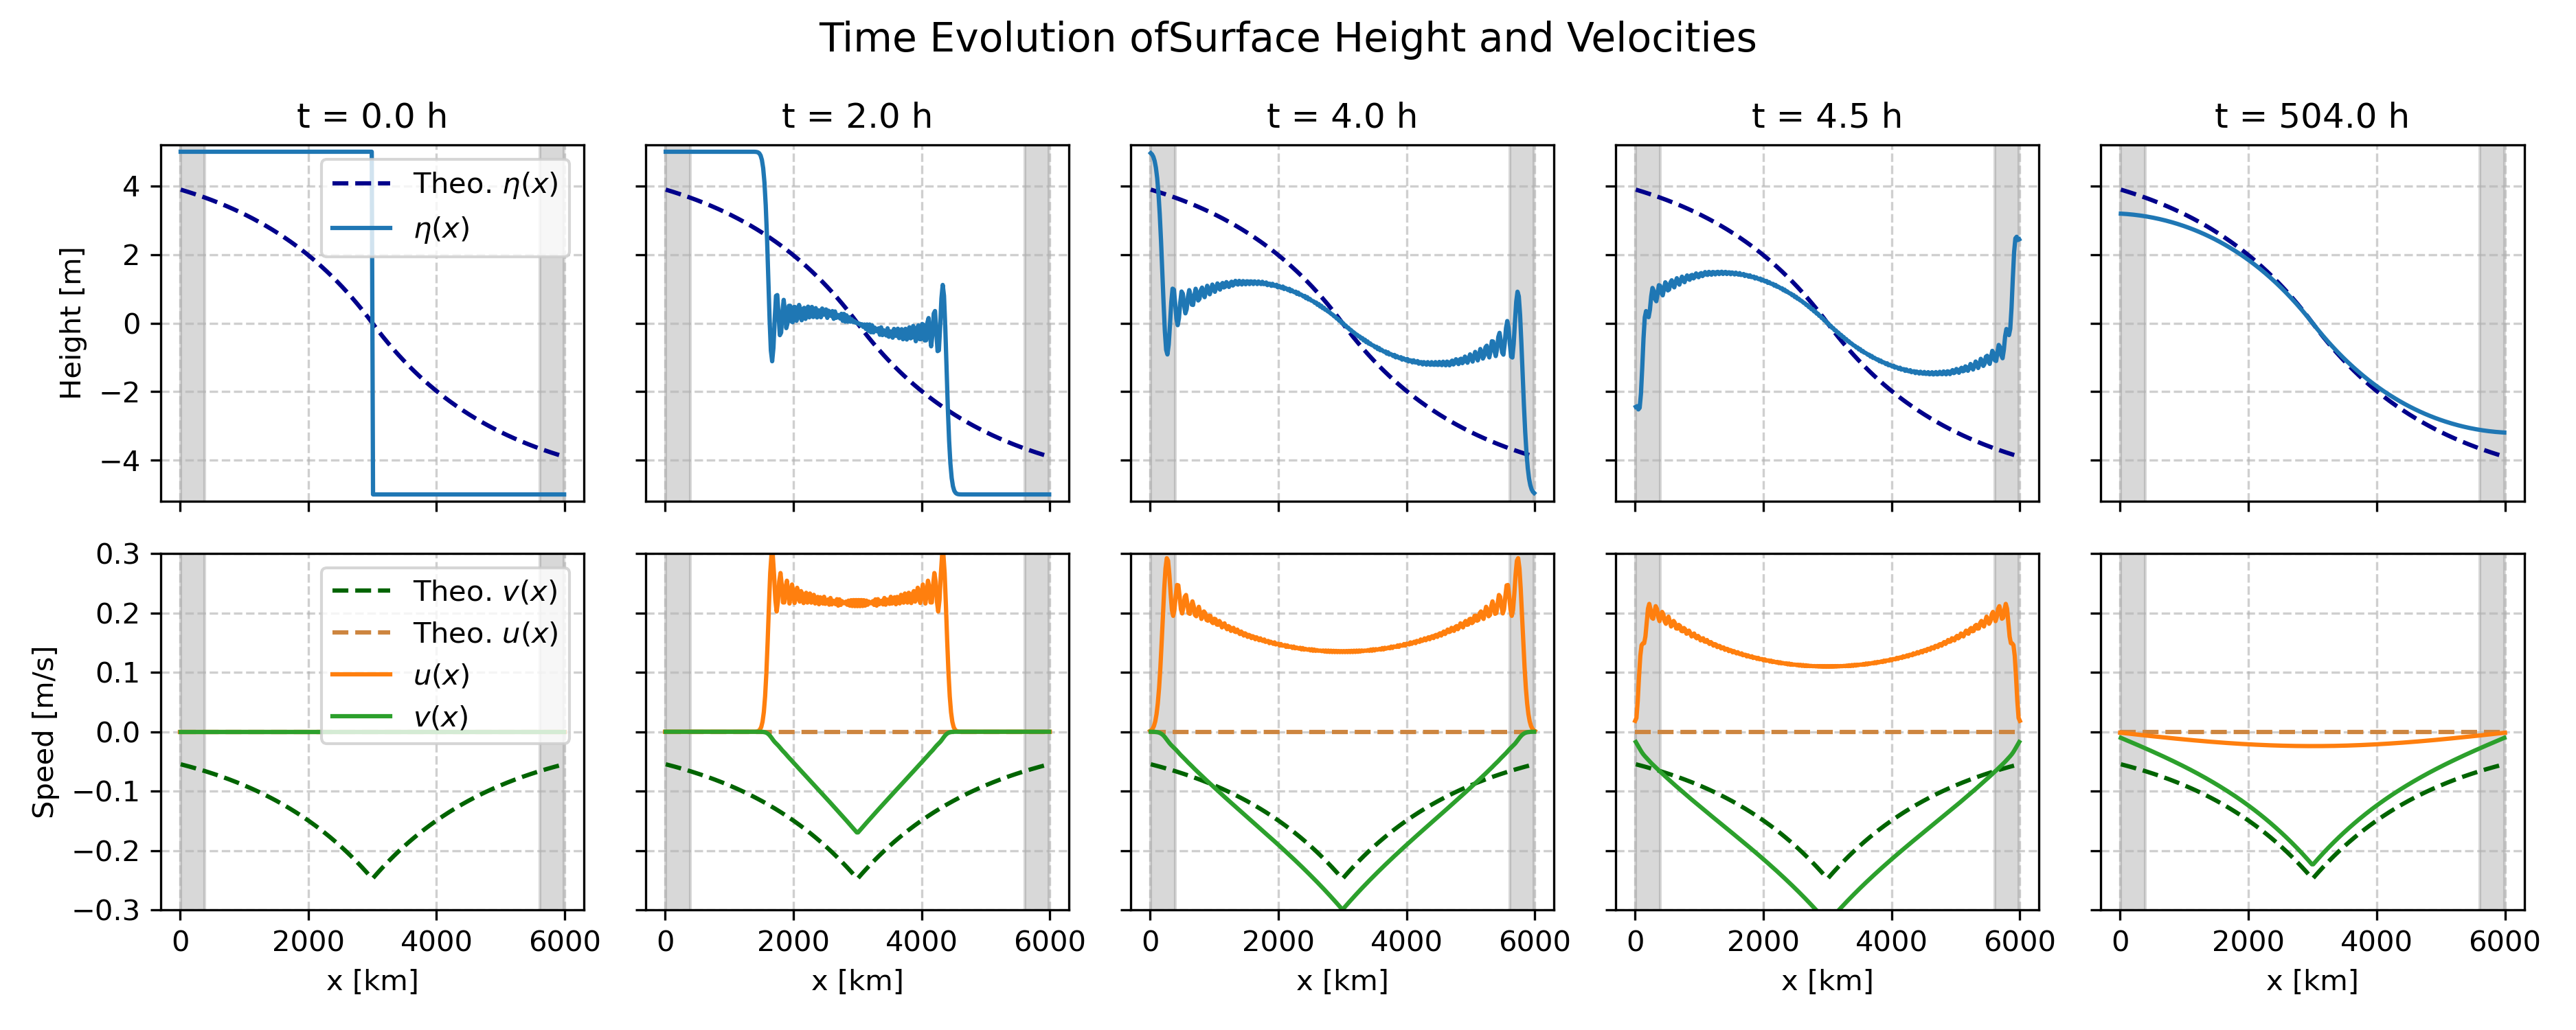
\includegraphics[width=0.9\textwidth]{Figures/graph.png}
    \caption{This figure shows the initial state of the model, the first few hours, and the final state. The grey area shows the location of the sponge. This model used a mean depth of $4000$ m, a Coriolis parameter of $10^{-4}$ s$^{-1}$, and a grid size of $6000$ km $\times$ $4500$ km.}
    \label{fig:graph}
\end{figure}

\begin{figure}[H]
    \centering    
    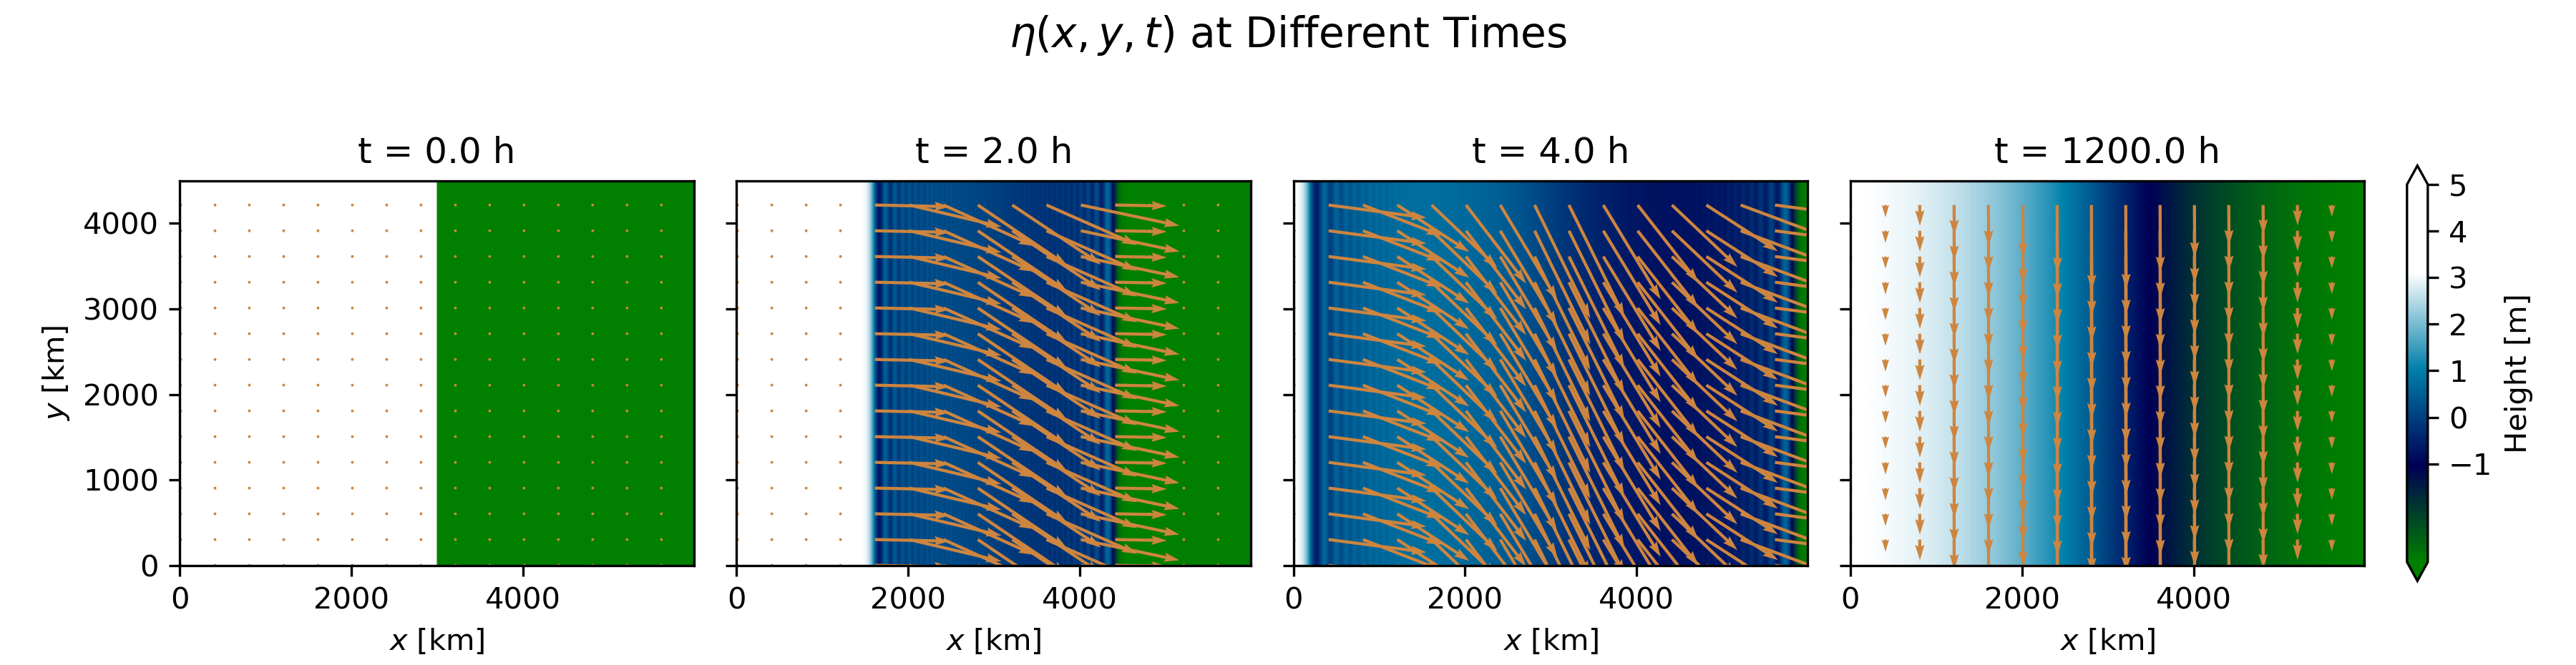
\includegraphics[width=\textwidth]{Figures/timesteps.png}
    \caption{This figure shows the initial state of the model, the first few hours, and the final state. Initially one can see fast moving waves disappearing by the sponge, but also that some are reflected. The final state showcases a clear hill-like shape.  }
    \label{fig:im}
\end{figure}

\begin{figure}[H]
    \centering    
    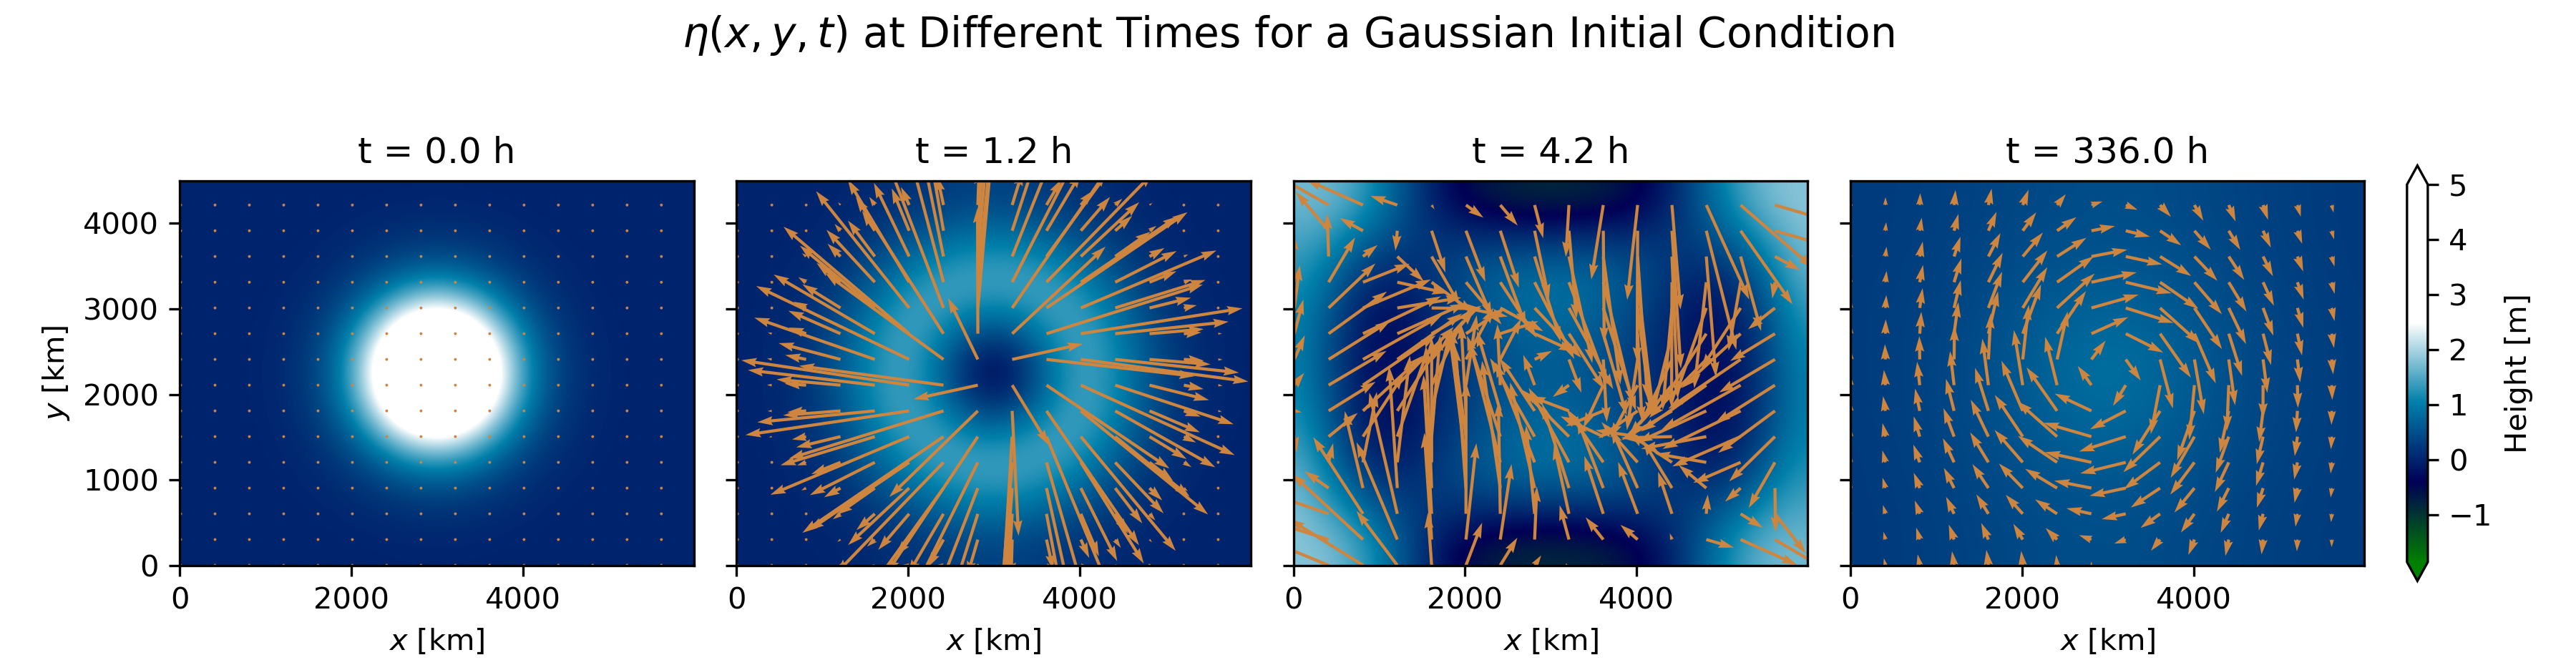
\includegraphics[width=\textwidth]{Figures/timesteps_gaussian.png}
    \caption{This figure shows the initial state of the model, the first few hours, and the final state for a gaussian initial condition. Here the initial condition was a bump in the free surface height, which is more smooth than the step initial condition. Note that the bump is positive while the rest remains at zero, thus the limit when $x\rightarrow\pm\infty$ is zero. Initially one can see fast moving waves disappearing by the sponge, but also that some are reflected. The final state showcases a clear anticyclonic high-pressure system in geostrophic balance.  }
    \label{fig:gaussian}
\end{figure}

\textbf{(iv)} Varying the Rossby radius of deformation $R$ by changing the Coriolis parameter $f$ and the mean depth $H$ can be seen in \autoref{fig:graph_comparison} and \autoref{fig:convergence}. In \autoref{fig:graph_comparison} one can see the final state for different choices of $f$ and $H$. One can see that the solution is a function of $R$, as the solution changes when $f$ and $H$ are changed. One can observe that a more spread out solution can be observed for larger $R$, as expected from the theory. Furthermore, since the model uses a finite grid of $6000$ km $\times$ $4500$ km, the larger Rossby radii are not captured by the model. Instead these become very flat in $\eta(x)$, since they need a large domain to reach their edge value $\pm\eta_0$. The smaller Rossby radii is well captured by the domain as seen in \autoref{fig:graph_comparison}. 

In \autoref{fig:convergence} the convergence towards the theoretical solution can be seen. There it also clear that when we use a smaller Rossby radii the model agrees well with the theoretically derived solutions (see \autoref{eq:solh} and \autoref{eq:solv}). Thus, one can see the convergence towards a accurate steady state solution when $t\rightarrow\infty$ for this smaller Rossby radii. For the larger Rossby radii, the agreement with the theoretical steady state is much worse. This make sense since these solutions were not captured by the model since the Rossby radius is close to, or even larger, then the domain size. Furthermore, one can note that it took longer time for the smaller Rossby radii models to converge to a steady state. This can be seen by the zonal velocity $u$ not reaching zero for these radii during the same timespan. 

The same behaviour can later be seen in the energy evolution plots shown in \autoref{fig:energy} and \autoref{fig:energy_large}. Simulations with smaller Rossby radii take longer time to converge toward geostrophic balance. One possible explanation is that the Rossby radius is not the main driver in this, but rather $H$. As $H$ increases, so does the speed of the Poincaré waves, which have a a speed of $c=\sqrt{gH}$. And instead looking at the size of $H$, one can see that a larger $H$ is what determines the time of convergence. These waves is what have to carry away the energy, and determine the adjustment and thus the convergence. There is also a small difference for the models with the same $H$, but different $f$. The reason for the lower Coriolis parameter converging faster may however simply be due to the lack of us capturing the entire solution in this finite domain. 

One note on the comparison between the theory and the numerical result is that even for the smaller Rossby radius, the numerical model is not 100\% like the theoretical one. Even here one can observe that the numerical solution is a little 'weaker' then the theoretical one. Thus, the numerical model experiences more energy loss then expected. In the theory energy can only be 'lost' though the propagation of the Poincaré waves. However, here we also have small scale dissipation, reflections at the walls, and as energy loss due to the sponge. 

\begin{figure}[H]
    \centering    
    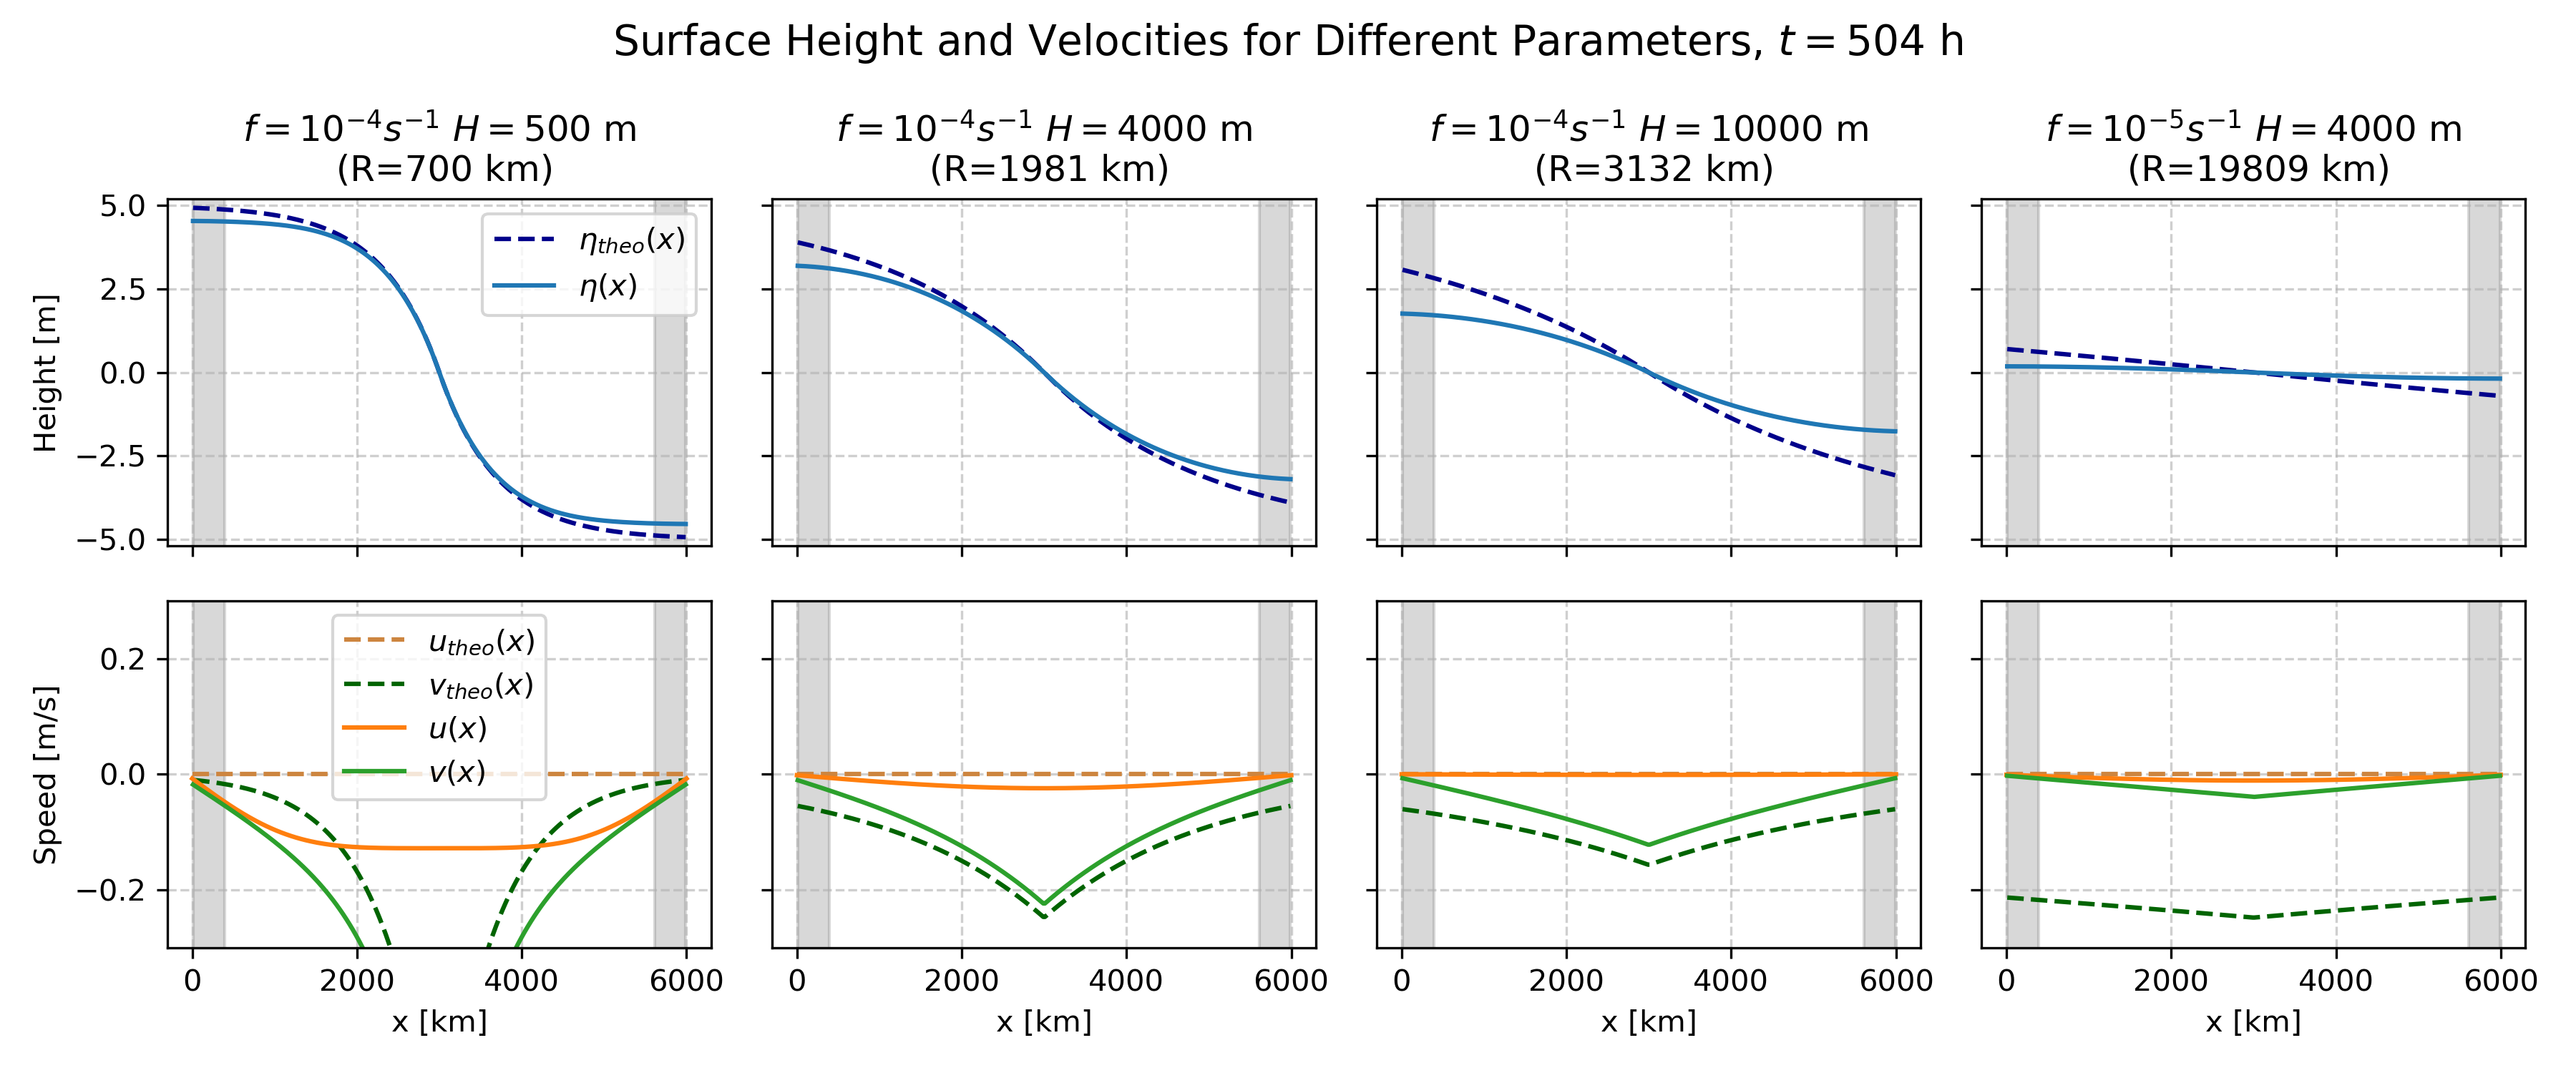
\includegraphics[width=0.9\textwidth]{Figures/graph_comparison.png}
    \caption{This figure shows the state at $t=504$h for different choices of coriolis parameter $f$ and mean depth $H$. The grey area shows the location of the sponge. The top row shows the free surface height, and the bottom row shows the meridional velocity.}
    \label{fig:graph_comparison}
\end{figure}


\begin{figure}[H]
    \centering    
    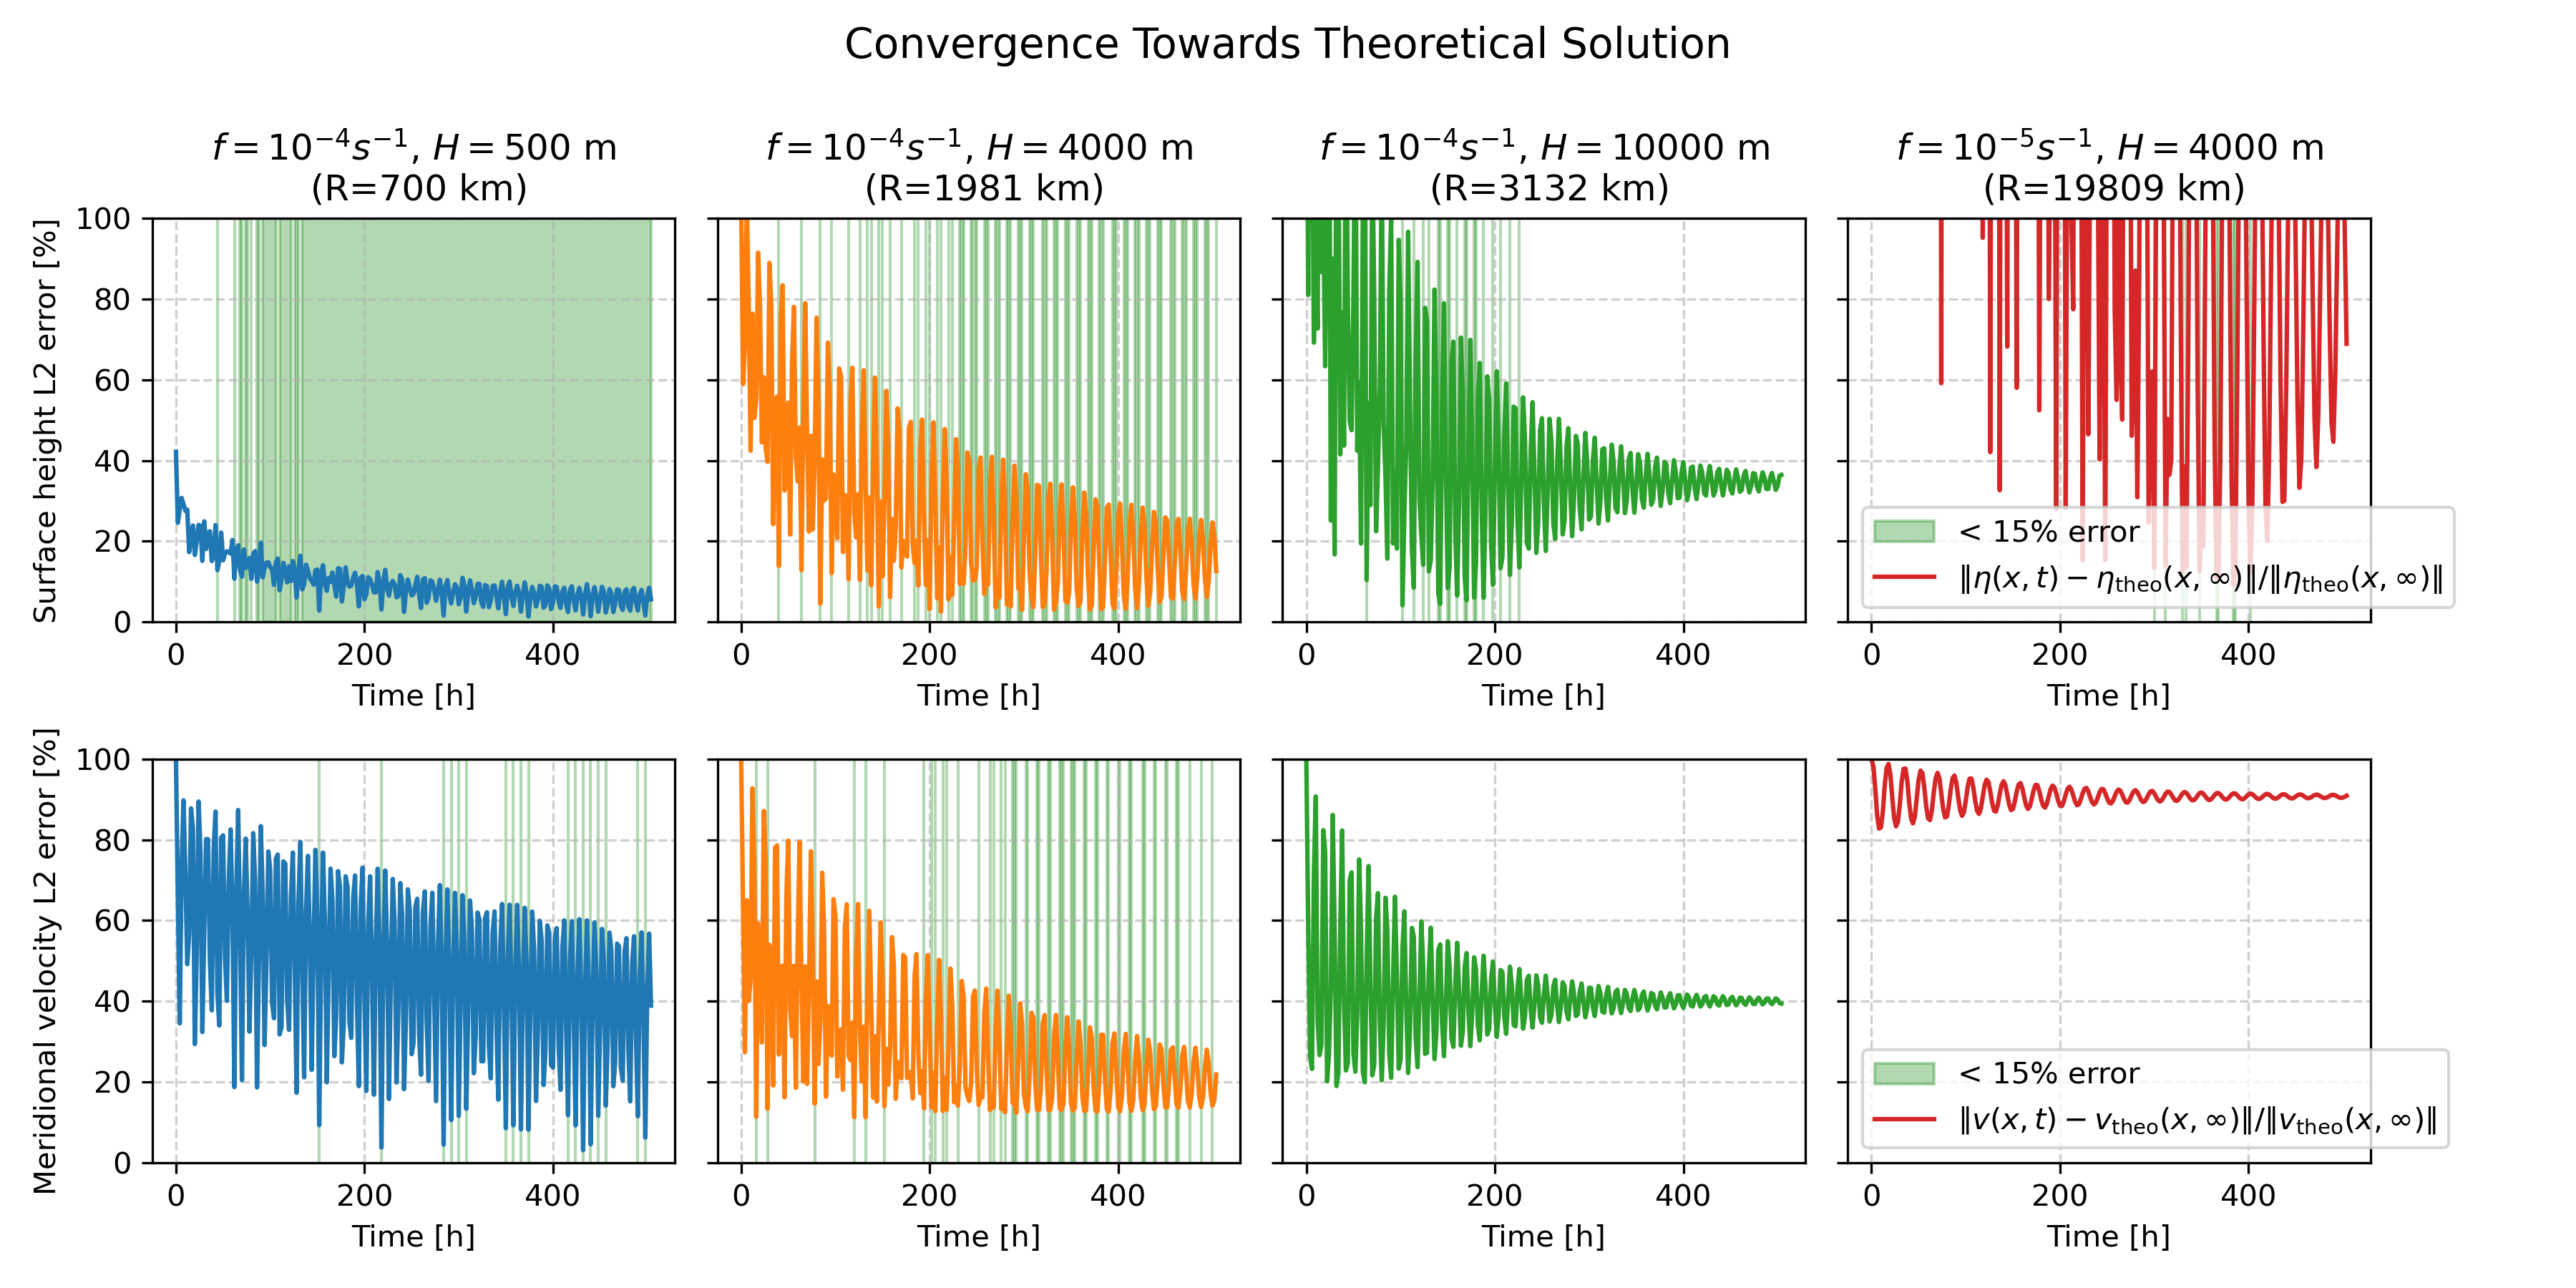
\includegraphics[width=0.9\textwidth]{Figures/convergence.png}
    \caption{This figure shows the convergence towards the theoretical solution for the different Rossby radii. The error between a numerical scheme and analytical solution can be quantified using the norm. For a vector $\mathbf{h}^n$, the $\ell_2$-norm is defined as $\|\mathbf{h}^n\| = \sqrt{ \frac{1}{N} \sum_{j=1}^{N} (h_j^n)^2 }.$ To obtain a dimensionless measure of the error, the relative error can be computed at time step $n$ as $\text{error}^n = \tfrac{\|\mathbf{h}_{\text{numerical}}^n - \mathbf{h}_{\text{analytical}}^n\|}{\|\mathbf{h}_{\text{analytical}}^n\|} $. The shaded green area shows where the data agrees well with the theoretical result. }
    \label{fig:convergence}
\end{figure}

\textbf{(v)} The choice of parameters were based on varying the model for different realistic parameters. The coriolis parameter is about $f\propto1e-4$ at the mid latitudes, but goes to zero close to the equator. Thus, close to the equator one would need a much bigger ocean to capture this phenomena, then if this where to happen in the midlatitudes. The oceans depth can also vary greatly, and was thus set to $10000$m and $500$m. This showed that shallower oceans does not have to be as large as a deep ocean to capture the same phenomena. 

Varying both the Coriolis and the mean ocean depth showed similar result to what was presented in the theory section. Decreasing the ocean mean depth $H$ to $500$m showed to make the solution more localised, and a larger magnitude $\abs{v}$. Increasing the depth to $10000$m showed to instead broaden the solution, and also lowered the magnitude $\abs{v}$. Lowering the Coriolis parameter to $f=1e-5$ showed a much broader solution, even broader then the increased ocean depth. However the theoretical magnitude remained the same as when a larger Coriolis parameter of $f=1e-4$ was used. However, this was not seen in the numerical model, where both the free surface height and velocity was lower then the theoretical solution. This can be connected to discussion above, where this very large Rossby radius needs a much larger domain to show the geostrophic adjustment. Thus, by varying the parameters the model showcased the characteristics explained by the theory. However, when a to large Rossby radius was chosen then the model showed a large discrepancy from the theoretically derived solution, as explained by the domain size. 
